\setlength{\columnsep}{3pt}
\begin{flushleft}
	\bigskip
	\begin{itemize}
		\item Every machine on internet needed to be update with newly added server entries in \textbf{/etc/hosts} file.
		\bigskip
		\item There was no kind of notification available for clients to know a new entry has been added.
		\bigskip		
		\item A single \textbf{/etc/hosts} file became large and very large, making it difficult to handle.
	\end{itemize}

	\paragraph{Solution: DNS server or nameservers}
	\begin{itemize}
		\item During the mid 1970's, \textbf{nameservers} came into place. 
		\bigskip
		\item Idea behind \textbf{nameservers} was to solve the problem of resolving hostname to numbers.
		\bigskip
		\item Nameserver, are also known as a \textbf{DNS server}.
		\bigskip
		\item DNS servers are mentioned in \textbf{/etc/resolv.conf} file.		
	\end{itemize}


	\newpage
	\paragraph{/etc/resolv.conf file}
	\begin{itemize}
		\item Lists nameservers that are used for DNS resolution. 
		\item This file contains a lines specifying the \textbf{"search domains"} and up to \textbf{three IP addresses of DNS server}. 
		\item Eg: Below resolv.conf have two \textbf{search domains} and \textbf{three DNS servers}:
		\begin{tcolorbox}[breakable,notitle,boxrule=-0pt,colback=black,colframe=black]
			\color{green}
			\fontdimen2\font=1em
			\# cat /etc/resolv.conf
			\newline
			\color{white}
			search us.mydomain.com mydomain.com
			\newline
			nameserver 192.168.154.3
			\newline
			nameserver 192.168.154.4
			\newline
			nameserver 10.216.106.3
			\fontdimen2\font=4pt
		\end{tcolorbox}
		\item If you are using DHCP, this file is automatically populated with DNS record issued by DHCP server.
		
	\end{itemize}

	\newpage
	\paragraph{/etc/nsswitch.conf file}
	\begin{itemize}
		\item This file defines, "Who should be consulted first for resolution of domain name, a DNS server or a /etc/hosts file?" 
		\bigskip
		\item Eg: Configuration setting \textbf{"hosts: files dns"} in this file means:
		\begin{itemize}
			\item \textbf{/etc/hosts} file will be checked first for resolution.
			\item If domain is still un-resolvable, DNS will then be consulted.
		\end{itemize}
		\begin{figure}[h!]
			\centering
			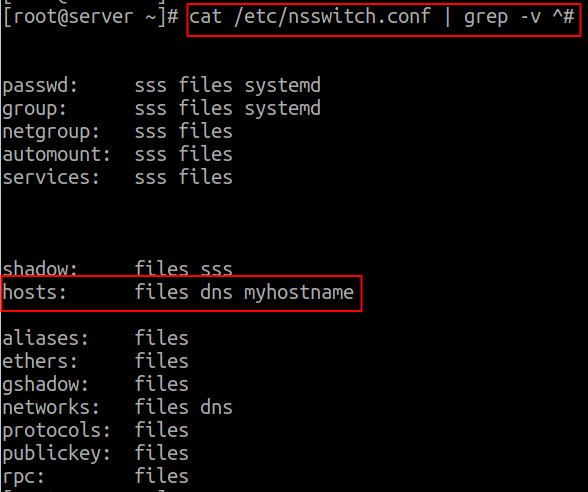
\includegraphics[scale=.45]{content/chapter3/images/ns.png}
			\caption{nsswitch file with hosts entry}
			\label{fig:ns}
		\end{figure}
		\item Note that DNS servers are mentioned in \textbf{/etc/resolv.conf}.
	\end{itemize}
	
	
	\newpage
	\bigskip
	\bigskip
	
	\begin{figure}[h!]
		\centering
		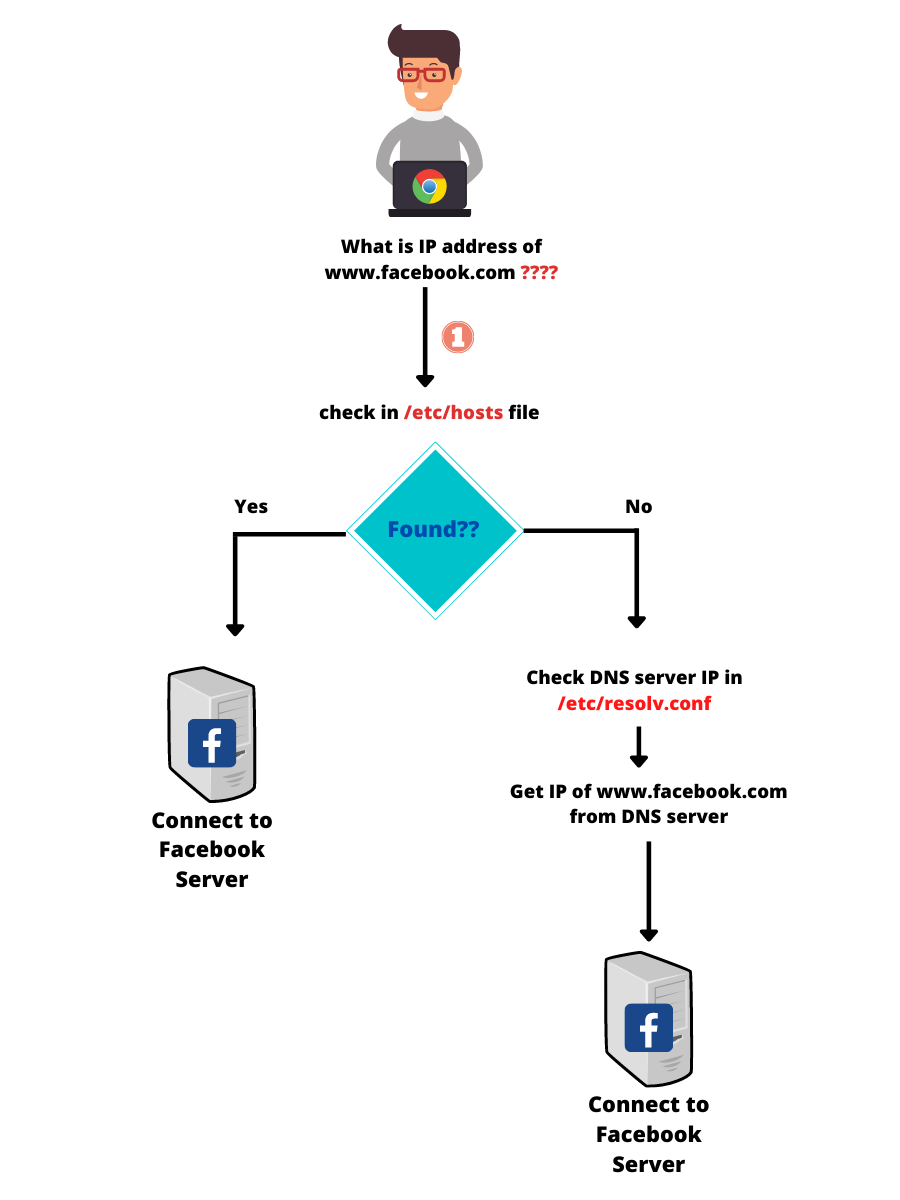
\includegraphics[scale=.6]{content/chapter3/images/hosts.png}
		\caption{Working of /etc/nsswitch.conf}
		\label{fig:dns_s}
	\end{figure}
	


\end{flushleft}

\newpage





